\chapter{Softwares para implementação}
\label{cap:softwares}

%Para comparar e selecionar o \textit{software} mais adequado para esta implementação utilizou-se uma técnica semelhante à descrita no artigo 
%de \cite{thome2013}. Neste artigo foi feita uma análise comparativa de ferramentas \textit{open source} de computação em nuvem. Sendo que, 
%foram criadas as seguintes características para fazer uma análise comparativa das ferramentas:
%interface, gerenciamento de energia, balanceamento de carga, rede, armazenamento, monitoramento, integração, virtualização, segurança, 
%escalabilidade e tolerância a falhas. Essas características são importantes para medir a qualidade e compatibilidade das ferramentas estudadas, 
%além de comparar a usabilidade das ferramentas.

%Usar metodologia MAH - Método Analítico Hierárquico \cite{geordano2014} NAO INICIALMENTE

Neste capítulo serão apresentadas as ferramentas que irão compor o ambiente de alta disponibilidade que foi proposto neste trabalho. A solução 
será baseada na utilização de virtualização e de \textit{softwares} de código aberto. Essa estrutura foi baseada nos trabalhos de 
\citet{goncalves2009}, \citet{reis2009} e \citet{zaminhani2008}. Os dois primeiros trabalhos implementam uma solução de alta disponibilidade 
através do uso de máquinas virtuais, com os mesmos objetivos deste trabalho. O terceiro autor utiliza uma técnica semelhante, porém implementada 
em apenas um serviço. Nestes trabalhos a estrutura é baseada em \textit{cluster}\footnote[1]{Pode-se definir \textit{cluster} como um grupo de 
computadores interligados por rede com o objetivo de aumentar o desempenho ou disponibilidade de um serviço \cite{freitas2005}}, onde é utilizado 
um \textit{software} responsável pela replicação de dados e um outro para o monitoramento e a gerência do \textit{cluster}. 

Para a escolha do \textit{software} de replicação de dados utilizou-se critérios que fossem compatíveis com a estrutura apresentada nos trabalhos
de \citet{goncalves2009} e \citet{reis2009}, e que fossem adequadas para o ambiente da empresa. Os critérios utilizados para a escolha do 
\textit{software} de replicação foram:
%As características que serão utilizadas para adotar o \textit{software} mais adequado para a implementação deste trabalho foram divididas em
%dois grupos e estão listadas abaixo.

\begin{itemize}
 \item Integração com virtualização: possibilidade de replicação dos dados das máquinas virtuais;
 \item \textit{Dual-primary}: suporte para leituras e escritas simultâneas em ambos os nós do \textit{cluster};
 \item Replicação em tempo real: replicação dos dados de forma instantânea e automática;
 \item Nível de replicação: possibilidade de replicação a nível de bloco ou de arquivo.
 %\item Número máximo de nós: quantidade de nós comportado pelo \textit{cluster}. Observa-se que para esse trabalho é necessário no mínimo dois.
\end{itemize}

Já os critérios utilizados para a escolha do \textit{software} de monitoramento e gerência do \textit{cluster} foram:
\begin{itemize}
 \item Suporte nativo à virtualização: possibilidade de monitorar e manipular máquinas virtuais;
 \item Migração de \acp{VM} em tempo real: suporte para a utilização de \textit{live migration}, ou seja, possibilita mover 
 uma \ac{VM} de um nó para outro sem reiniciá-la;
 \item \textit{Failover} e \textit{failback} automáticos: suporte para a movimentação automática dos serviços do nó que falhou para um outro 
 nó disponível.
 %\item Sincronismo de configuração entre os nós: configuração do \textit{cluster} pode ser alterada em qualquer nó, ou seja, ocorre a replicação
 %da configuração para todos os nós do \textit{cluster}.
\end{itemize}

\section{Softwares para a replicação de dados}
\label{section:toolrepl}

A replicação de dados pode ser realizada de diferentes formas, podendo ser a nível de aplicação ou até mesmo a nível de \textit{hardware}.
Dependendo do objetivo pode-se utilizar uma replicação através de um \ac{RAID}\footnote[1]{RAID é usado para melhorar a confiabilidade e o
desempenho no armazenamento de dados, fazendo a redundância de dados em um conjunto de discos rígidos \cite{zaminhani2008}.}. 
Essa solução é eficaz para garantir que o sistema não fique indisponível em caso de falha nos discos\footnote[2]{Lembrando que essa solução é 
utilizada no ambiente atual para aumentar a disponibilidade dos servidores.} rígidos, porém não garante a disponibilidade quando um 
\textit{software} ou algum outro componente de \textit{hardware} falhar \cite{zaminhani2008}.
%\ac{RAID} \cite{tanenbaum2009sistemas}

A solução de replicação a ser adotada neste trabalho consiste em um espelhamento de dados através da rede. Essa solução permite a sincronização 
dos dados de um servidor para outro em tempo real.
Nas próximas seções tem-se uma descrição dos \textit{softwares} de replicação de dados que foram estudados, bem como as funcionalidades 
suportadas pelos mesmos.

% \subsubsection{Ceph RBD}
% \label{section:cephrbd}
% O \textit{Ceph RBD} \cite{cephrbd} faz parte do projeto \textit{Ceph} \cite{ceph}. O \textit{Ceph RBD} é responsável por prover acesso dos 
% dispositivos de bloco que estão distribuídos ou replicados em um \textit{cluster}. Sua arquitetura é composta por um nó administrador, onde será
% centralizado a gerência do \textit{cluster}, e deve conter no mínimo dois nós para armazenamento (\textit{Ceph OSD}) e monitoramento 
% (\textit{Ceph Monitor}). Conceito de n OSDs e n+1 monitors.
% \cite{ceph}.

\subsection{\aca{DRBD}}
\label{section:drbd}
O \ac{DRBD} é um projeto de código aberto desenvolvido pela \textit{LINBIT} \cite{drbd}.
Esse \textit{software} é uma solução de replicação de dispositivos de armazenamento, ou seja, esse permite a duplicação de um dispositivo de bloco 
(geralmente um disco rígido) em um servidor remoto. O \ac{DRBD} é implementado através de um módulo do \textit{kernel} \textit{Linux}. 
Na Figura \ref{fig:drbd_basic} tem-se dois servidores com seus respectivos discos rígidos, \textit{hda1} e 
\textit{hda3}, formando um \textit{cluster}, sendo que esses discos estão sincronizados através da rede. Desta forma, todas as operações de escrita 
que são realizadas no disco rígido do nó primário são replicadas no nó secundário \cite{zaminhani2008}.

\begin{figure}[h!]
 \centering
 \fcolorbox{black}{white}{
  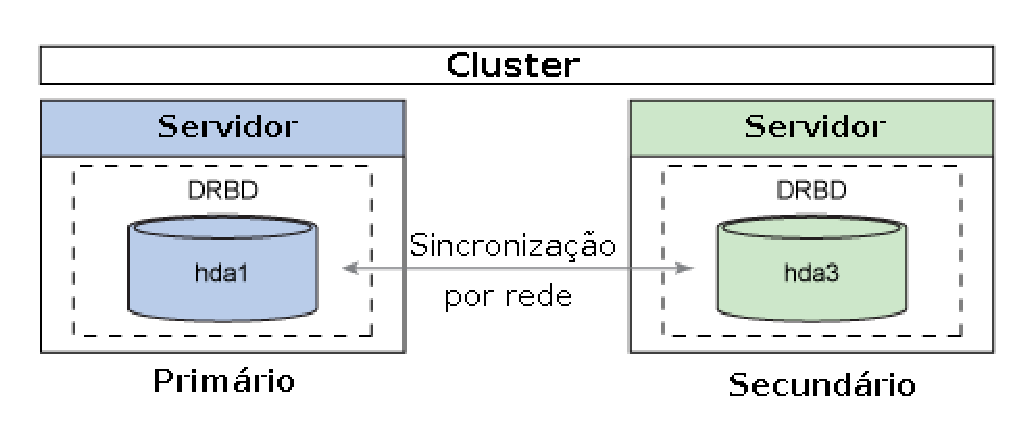
\includegraphics[width=300px]{img/drbd_basic.eps}
 }
 \caption{Exemplo do modelo \textit{master-slave} do \ac{DRBD}.}
 Fonte: \citet{jones2010}
 \label{fig:drbd_basic}
\end{figure}

O \ac{DRBD} pode ser configurado dos seguintes modos \cite{drbd}:
\begin{itemize}
 \item \textit{Single-primary} ou \textit{master-slave}: neste modo apenas um nó do \textit{cluster} pode ser o nó primário, sendo que somente
 o nó primário terá permissão para acessar o dispositivo, ou seja, somente ele poderá fazer operações de leitura e escrita. De fato, neste modo 
 o nó secundário terá apenas uma réplica dos dados;
 \item \textit{Dual-primary} ou \textit{dual-master}: neste modo existem dois nós primários, nos quais podem ser realizadas operações de leitura e 
 escrita de forma simultânea. Porém, este modo necessita de um sistema de arquivos compartilhados, sendo que neste caso podem ser utilizados os
 sistemas de arquivos \ac{GFS} \cite{gfs} e \ac{OCFS2} \cite{ocfs2}.
\end{itemize}

\subsection{GlusterFS}
\label{section:glusterfs}
O \textit{GlusterFS} \cite{glusterfs} é um sistema de arquivos distribuídos mantido pela \textit{Gluster community}. Este utiliza uma estrutura 
de \textit{cluster} e o seu principal objetivo é a escalabilidade, ou seja, este possui funcionalidades que facilitam ampliar a capacidade 
do \textit{cluster} a partir da inclusão de novos nós.

\begin{figure}[h!]
 \centering
 \fcolorbox{black}{white}{
  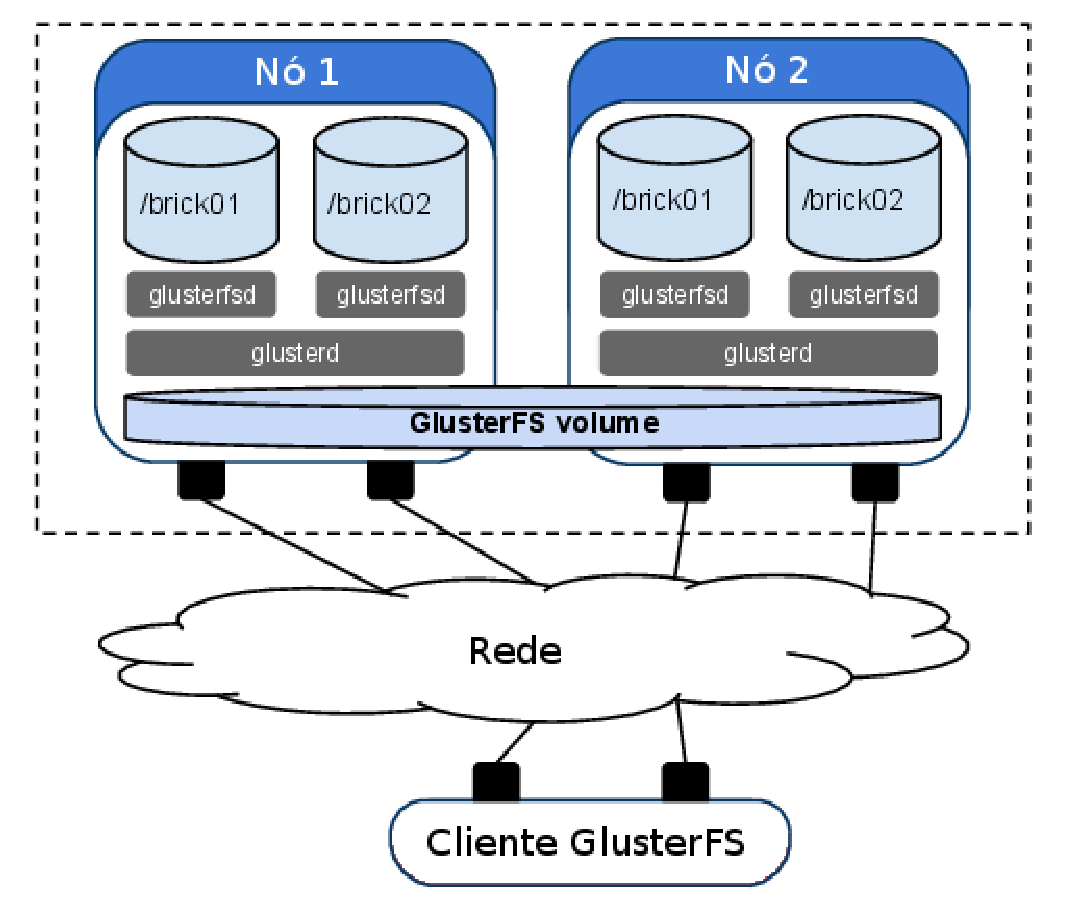
\includegraphics[width=280px]{img/glusterfs.eps}
 }
 \caption{Modelo do \textit{GlusterFS}.}
 Fonte: \citet{davies2013}
 \label{fig:glusterfs}
\end{figure}

Na Figura \ref{fig:glusterfs} tem-se um exemplo de dois nós, onde cada nó possui dois discos rígidos, que são denominados \textit{bricks}. 
A partir dos \textit{bricks}, o \textit{GlusterFS} constrói um volume lógico que é disponibilizado através da rede para todos os clientes. 
A organização destes \textit{bricks} vai depender do objetivo da aplicação, sendo que uma das formas é a replicação. 
Os diferentes tipos de configurações são \cite{glusterfs}:
\begin{itemize}
 \item Volume distribuído: neste modo os arquivos são distribuídos entre os diferentes \textit{bricks} dos nós. O objetivo deste tipo de 
 configuração é ampliar a capacidade de armazenamento. Neste modo, não se tem uma preocupação com a redundância de dados, sendo que no caso de uma
 falha em um dos nós, haverá uma perda de todos dados;
 \item Volume replicado: neste modo os arquivos são replicados entre os \textit{bricks}, desta forma, tem-se uma redundância, uma vez que no caso
 de uma falha em um \textit{brick}, não haverá perda de dados;
 \item Volume distribuído e replicado: este é uma combinação dos dois tipos de volumes anteriores. Neste caso, é feita a distribuição 
 e a replicação dos arquivos entre os nós;
 \item Volume listrado: neste modo de configuração ocorre a distribuição de um mesmo arquivo entre os \textit{bricks}, ou seja, um arquivo é 
 dividido entre os \textit{bricks}. Esse tipo é normalmente utilizado para o armazenamento de arquivos muito grandes e para garantir um melhor 
 balanceamento de carga em sistemas com muito acesso à disco. Neste tipo de volume não se tem nenhuma forma de replicação de dados;
 \item Volume distribuído e listrado: este modo de volume é uma combinação do distribuído e do listrado. Neste modo é feita a divisão do arquivo 
 entre \textit{bricks} distintos, sendo que estes são replicados.
\end{itemize}

\subsection{Rsync}
\label{section:rsync}
O \textit{Rsync} \cite{rsync} é um \textit{software} desenvolvido e mantido por \textit{Wayne Davison}. Esse \textit{software} provê uma rápida
transferência de arquivos, ou seja, ele faz a sincronização de arquivos transferindo-os de um servidor de origem para um servidor de destino. 
A Figura \ref{fig:rsync} apresenta o funcionamento do \textit{Rsync}, observa-se nesta figura que a replicação só é realizada em arquivos 
que foram alterados ou que ainda não existem no servidor de destino. Além disso, o \textit{Rsync} permite uma replicação completa, 
sendo que neste caso os arquivos já existentes são sobrescritos.

\begin{figure}[h!]
 \centering
 \fcolorbox{black}{white}{
  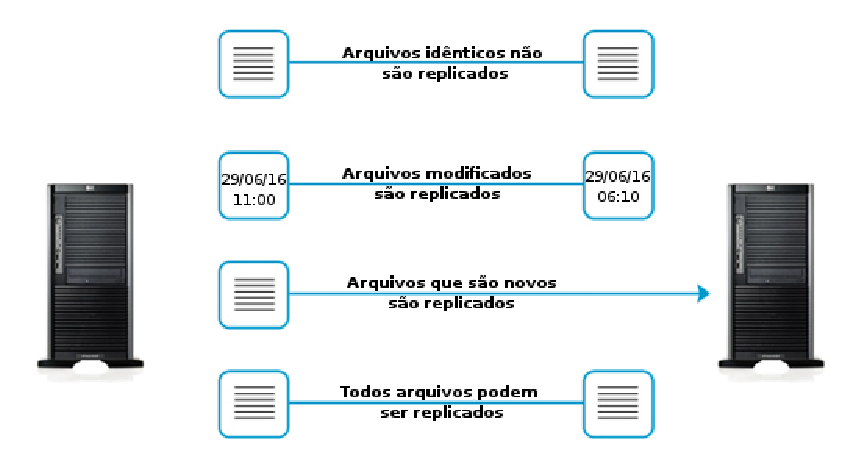
\includegraphics[width=370px]{img/rsync.eps}
 }
 \caption{Transferência de arquivos através do \textit{Rsync}.}
 Fonte: \citet{lopez2012}
 \label{fig:rsync}
\end{figure}

%Algoritmo \cite{tridgell98}

O \textit{Rsync} pode ser configurado como servidor, o que permite que vários clientes possam sincronizar seus arquivos com ele. 
Além disso, a sincronização pode ser feita de cliente para cliente, utilizando o protocolo \ac{SSH} para a transferência ou através de 
\textit{sockets}. Destaca-se que o \textit{Rsync} não faz uma sincronização em tempo real, ou seja, esse só realiza a sincronização a partir de 
uma ação de um operador, como por exemplo, a execução de um comando.

% Ceph RBD
% Swift open stack
% https://wiki.freebsd.org/HAST

\newpage
\subsection{Comparativo entre os softwares de replicação de dados}
\label{section:replicacaoescolhido}

Na Tabela \ref{tab:replicacao} tem-se uma comparação entre os \textit{softwares} de replicação apresentos anteriormente. O \textit{software} 
adotado para realizar a replicação de dados foi o \ac{DRBD}, pois esse permite a configuração \textit{dual-primary} e também \textit{master-slave}, 
além de suportar a replicação de dados das máquinas virtuais e permitir a replicação a nível de bloco. Além disso, esse \textit{software} 
permite a ressincronização dos dados de forma automática em caso de uma falha \cite{drbd}.

\begin{table}[h!]
\caption{Comparação ferramentas de replicação de dados.}
\label{tab:replicacao}
\begin{center}
\begin{tabular}{|l|p{3.5cm}|p{3.5cm}|p{2cm}|}\hline
\textbf{Critério} & \textbf{DRBD} & \textbf{GlusterFS} & \textbf{Rsync} \\\hline
Integração com virtualização & Sim & Sim & Não \\\hline
Dual-primary & Sim & Sim & Não \\\hline
Replicação em tempo real & Sim & Sim & Não \\\hline
Nível de replicação & Bloco & Arquivo & Arquivo \\\hline
%Número máximo de nós & 16 & 64 & Ilimitado \\\hline
Distribuições Linux & Suse, Debian, CentOS, Red Hat, Ubuntu & Debian, CentOS, Red Hat, Fedora, Ubuntu & Todas \\\hline
\end{tabular}
\end{center}
\end{table}

O \textit{GlusterFS} poderia ser utilizado, porém este faz uma replicação a nível de arquivo, desta forma esse \textit{software} não é adequado 
para uma solução de alta disponibilidade baseada em virtualização. E, por fim, o \textit{Rsync} não pode ser utilizado pois esse não executa 
uma replicação em tempo real, além de não ter sido desenvolvido para ser utilizado em conjunto com a virtualização.

%Pode-se perceber que o \textit{Ceph RBD} não possui a opção de
%\textit{master-slave}. Esse \textit{software} necessita de um \textit{hardware} adicional para sua administração. 

%https://www.reddit.com/r/linux/comments/1qwarp/drbd_vs_glusterfs/
% glusterfs mais escalável, simples de administrar
% drbd melhor eficiência(acredito) nível de bloco, confiável(10 anos develop)

% drbd: 2 nodes na versão 8 e 16 nodes por stacking / 16 nodes na versão 9

% drbd dispositivo primário e secundário zaminhani2008
% Segundo (ELLENBERG, 2007), a partir da versão 8 do DRBD é possível que,
%dependendo da aplicação, a execução ocorra em todos os nós do cluster
%simultaneamente (Ativo/Ativo). Para tornar isso possível é necessária a
%utilização de um sistema de arquivos exclusivo para cluster, como o OCFS2 6 e o
%GFS 7 por exemplo. Como a abordagem deste trabalho é cluster de alta
%disponibilidade, a utilização do DRBD no modo Ativo/Ativo não será discutida.

% glusterfs https://raobharata.wordpress.com/2012/10/29/qemu-glusterfs-native-integration/
% melhor performance com disco utilizando protocolo gluster file=gluster://path/to

% ceph http://docs.ceph.com/docs/master/start/intro/
% necessita mínimo 3 monitores com osd, outra para administração
% precisa openstack + nova
% http://www.server-world.info/en/note?os=Ubuntu_14.04&p=ceph
% https://elkano.org/blog/live-migration-openstack-ubuntu-14-04/

\section{Softwares para o gerenciamento do cluster}
\label{section:toolcluster}

Para que seja possível implementar uma solução de alta disponibilidade é necessário organizar os servidores em uma estrutura de \textit{cluster},
sendo assim, é interessante a utilização de \textit{softwares} que facilitem o gerenciamento deste \textit{cluster}. Esses \textit{softwares} 
são conhecidos como \ac{CRM}, e permitem detectar falhas em um nó, sendo elas de \textit{hardware} ou de serviços. 

Após a detecção de uma falha, os \textit{softwares} de gerenciamento de \textit{cluster} executam operações de \textit{failover} e 
\textit{failback}. O \textit{failover} é um processo no qual um outro servidor recebe os serviços que estavam executando no servidor que falhou. 
Já no processo de \textit{failback} tem-se um retorno dos serviços para o servidor de origem quando este estiver disponível. Esse processo ocorre 
após o \textit{failover}, sendo que ele é opcional \cite{bassan2008}. Nas próximas seções será feita uma breve descrição dos \textit{softwares} de 
gerenciamento de \textit{cluster} que foram estudados.

% \subsubsection{Ceph}
% \label{section:ceph}
% O \textit{Ceph} \cite{ceph} é uma ferramenta com foco no armazenamento de dados distribuídos. Esta ferramenta tem foco em \textit{cluster} 
% de armazenamento, sendo assim ela necessita de outra ferramenta para gerenciar as máquinas virtuais, como por exemplo \textit{OpenStack} 
% \cite{openstack}. Sua arquitetura é composta por um nó administrador, onde tem-se a gerência do \textit{cluster}, e no mínimo dois 
% nós, sendo um para o armazenamento (\textit{Ceph OSD}) e um para o monitoramento (\textit{Ceph Monitor}) e o processamento (\textit{Ceph MDS}) \cite{ceph}.

\subsection{Ganeti}
\label{section:ganeti}
O \textit{Ganeti} \cite{ganeti} é um \textit{software} desenvolvido pelo \textit{Google}, utilizado como um gerenciador de \textit{cluster} 
baseado em virtualização. De fato, esse foi desenvolvido especificamente para ambientes de virtualização e suporta os hipervisores 
\ac{KVM} \cite{kvm} e \textit{Xen} \cite{xen}. 

\newpage
Na Figura \ref{fig:ganeti_arquitetura} tem-se um exemplo de um \textit{cluster} com uma arquitetura do \textit{Ganeti}, sendo que este 
\textit{cluster} é composto por um nó \textit{master}, que armazena as configurações e gerencia o \textit{cluster}, e um nó 
\textit{master candidate}, para o caso de uma falha no nó \textit{master}. Além disso, a arquitetura é formada por vários nós \textit{slaves}. 
Destaca-se que no \textit{Ganeti} todos os nós são responsáveis por prover o ambiente de virtualização e armazenar os dados das \acp{VM}, 
sendo que cada nó pode possuir uma ou mais instâncias de \acp{VM}. Em cada instância das \acp{VM} configura-se dois nós, que são: o nó primário, 
onde a instância da \ac{VM} será executada; e o nó secundário, que será utilizado no caso de uma falha no nó primário.
Além disso, as instâncias das \acp{VM} também podem ser migradas de um nó para outro de forma manual. 

\begin{figure}[h!]
 \centering
 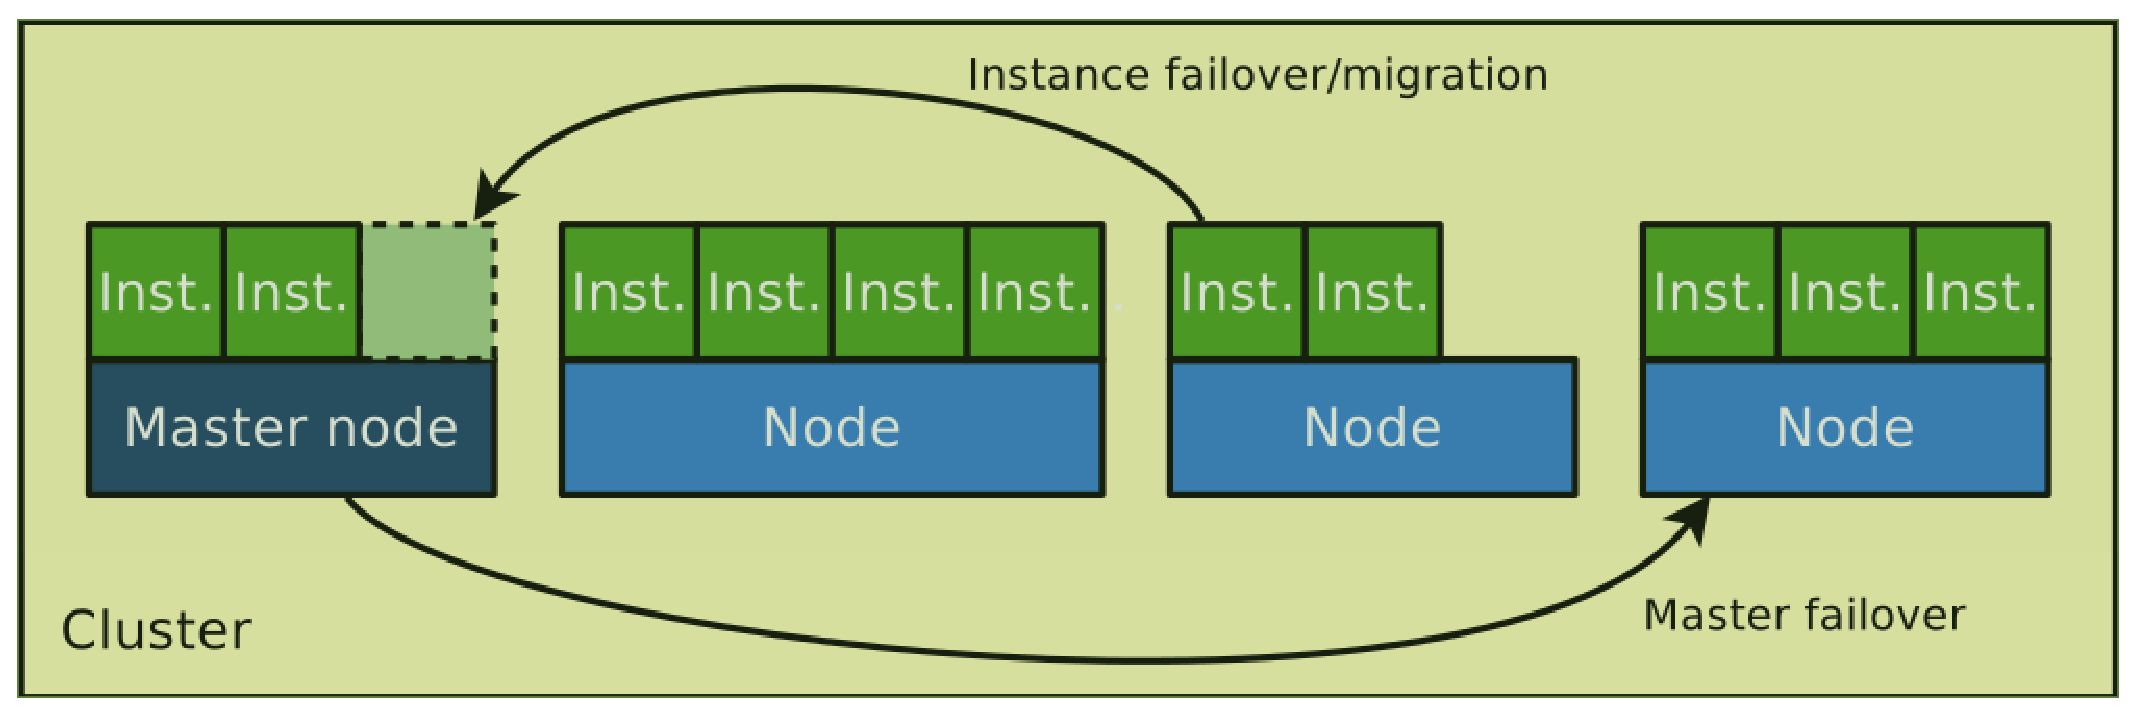
\includegraphics[width=380px]{img/ganeti_arquitetura.eps}
 \caption{Arquitetura do \textit{Ganeti}.}
 Fonte: \citet{carvalho2011}
 \label{fig:ganeti_arquitetura}
\end{figure}

De forma resumida, as principais funcionalidades do \textit{Ganeti} são \cite{ganeti}:
\begin{itemize}
 \item Criação de instâncias de \acp{VM};
 \item Gerenciamento do armazenamento das instâncias;
 \item Iniciar e finalizar instâncias, além de efetuar a migração das \acp{VM} entre os nós.
\end{itemize}

% ganeti pode ser usado com ceph rdb (RADOS Cluster), ou drbd, ou gluster

\subsection{Heartbeat}
\label{section:heartbeat}
O \textit{Heartbeat} é um subprojeto do \textit{Linux-HA} \cite{linuxha}, que desenvolve soluções de alta disponibilidade.
Esse subprojeto é uma aplicação que envia pacotes \textit{keepalive}\footnote{\textit{Keepalive} significa mantenha vivo, são sinais 
enviados em uma determinada frequência para verificar se a comunicação esta ativa.} \textit{\ac{UDP}}, 
através da rede, para outras aplicações \textit{Heartbeat}. Esses pacotes possuem como objetivo verificar se uma aplicação está ativa.
Destaca-se que esse \textit{software} pode ser utilizado para alta disponibilidade em ambientes de virtualização \cite{reis2009}.
Na Figura \ref{fig:heartbeat} tem-se uma ilustração mostrando a execução do \textit{Heartbeat} em dois servidores sobre as interfaces de rede 
dedicadas (identificadas na figura como \textit{ethX}).
Neste caso, se o nó secundário deixar de receber os sinais do nó primário, este irá se tornar o nó primário, e iniciará o processo de 
\textit{failover}. 
%com isso, ele receberá o \ac{IP} virtual (\textit{192.168.50.3}) e iniciará os serviços previamente configurados.
\begin{figure}[h!]
 \centering
 \fcolorbox{black}{white}{
  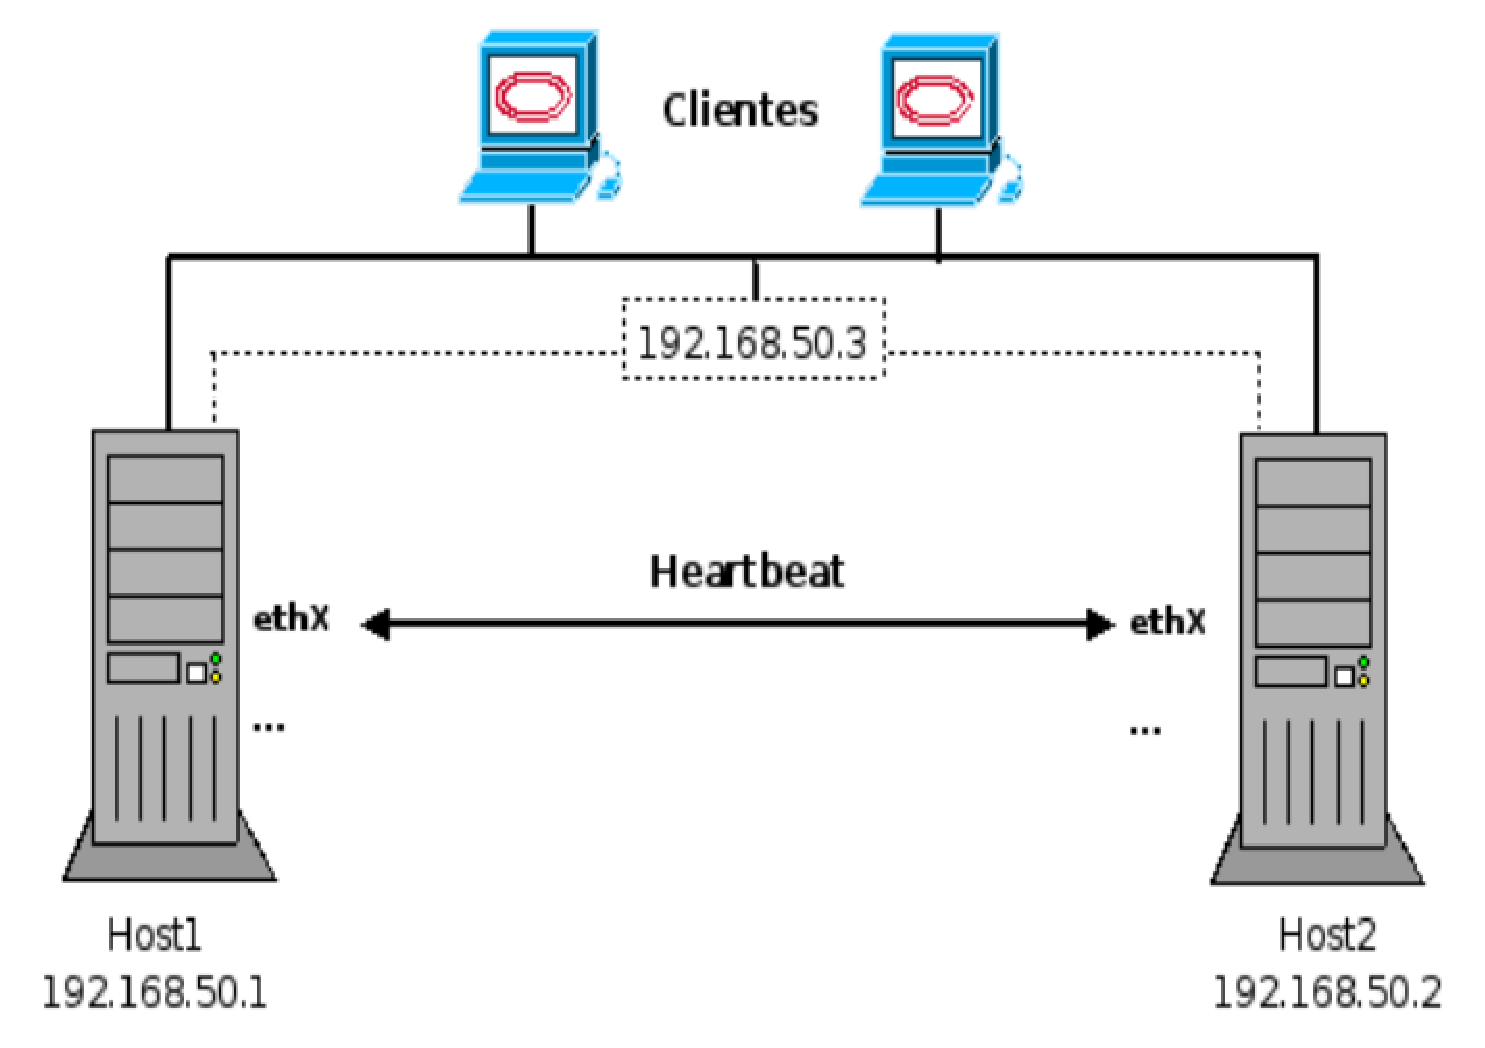
\includegraphics[width=280px]{img/heartbeat.eps}
 }
 \caption{Arquitetura do \textit{Heartbeat}.}
 Fonte: \citet{zaminhani2008}
 \label{fig:heartbeat}
\end{figure}

\newpage
De forma resumida, as principais funcionalidades do \textit{Heartbeat} são \cite{clusterlabs}:
\begin{itemize}
 \item Enviar mensagens entre os nós para a detecção de falhas;
 \item Efetuar os processos de \textit{failover} e \textit{failback};
 \item Iniciar e finalizar serviços nos nós;
\end{itemize}

%exemplo de implementacao heartbeat com virtualizacao = \cite{reis2009}

\subsection{Pacemaker}
\label{section:pacemaker}
O \textit{Pacemaker} \cite{pacemaker} é um projeto de código aberto mantido pela \textit{ClusterLabs}, e teve como origem uma necessidade 
de realizar um aperfeiçoamento do \textit{software} \textit{Heartbeat} \cite{heartbeat}. 
O \textit{Pacemaker} pode ser definido como um \textit{software} de recuperação de falhas a nível de serviço \cite{perkov2011}. 
Frequentemente, esse \textit{software} é utilizado juntamente com outros \textit{softwares} que fazem os registros dos nós e troca de mensagens entre os nós do 
\textit{cluster}, sendo que os \textit{softwares} que podem ser integradas com o \textit{Pacemaker} são \cite{pacemaker}:
\begin{itemize}
 \item \textit{Corosync} \cite{corosync}: derivou do projeto \textit{OpenAIS} e é responsável pelo processo de registro dos nós e pelo processo 
 de \textit{failover};
 %bloqueios distribuídos (utilizados para implementar \ac{LVM} \cite{lvm}, \ac{GFS}, e \ac{OCFS2}). 
 \item \textit{Heartbeat}: responsável pelo envio de mensagens entre os nós do \textit{cluster}, além de inicializar e finalizar os serviços.
\end{itemize}
% outras ferramentas cMAN e Apache Qpid

%Modelos Active/Passive, N+1, N TO N, Split Site

Na Figura \ref{fig:pacemaker_tools} tem-se a arquitetura do \textit{Pacemaker}. Como pode ser observado na camada inferior tem-se os nós do 
\textit{cluster}. Nas duas camadas acima tem-se o \textit{software} de envio de mensagens e o \textit{Pacemaker}, respectivamente. 
Por fim, tem-se os serviços, que serão executados no \textit{cluster}.

\begin{figure}[h!]
 \centering
 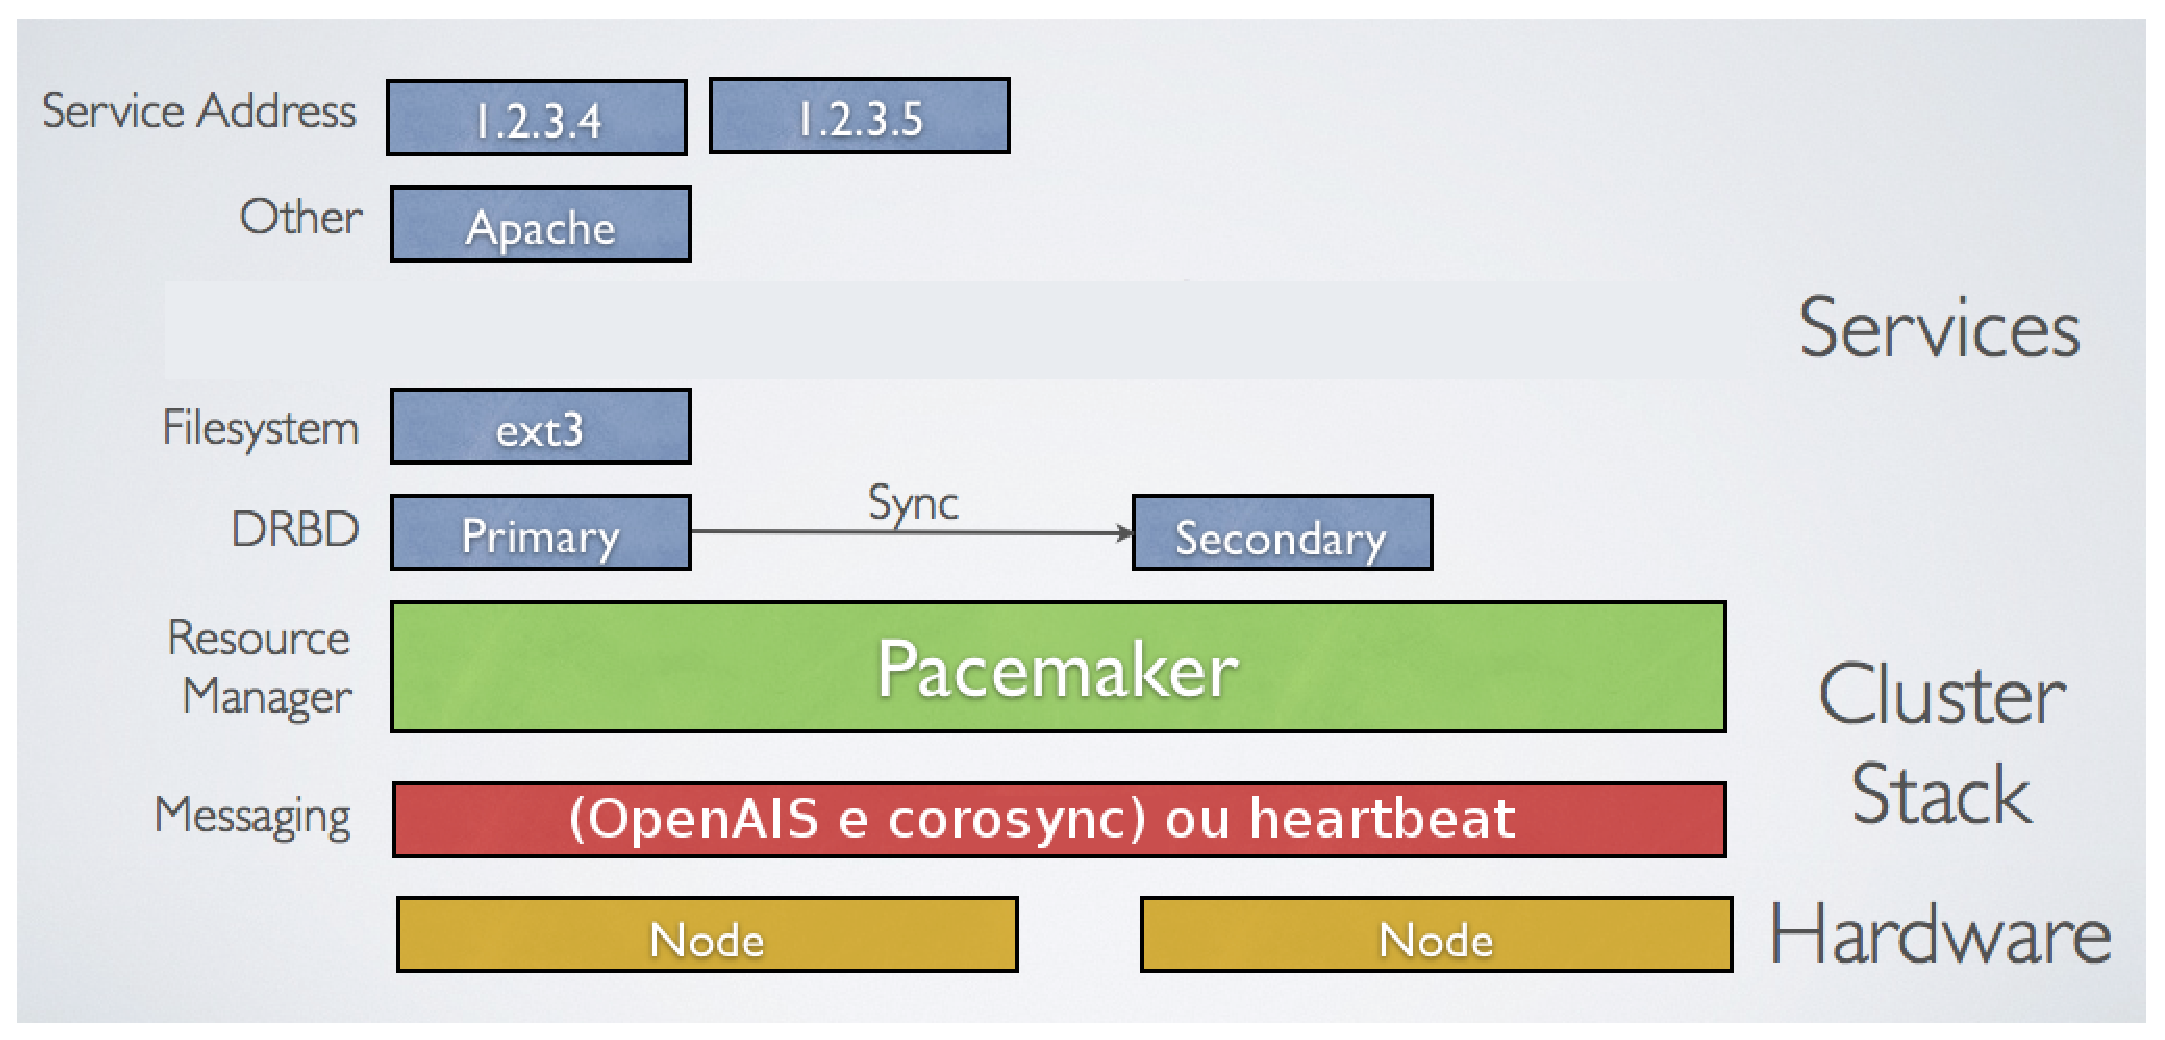
\includegraphics[width=380px]{img/pacemaker_tools.eps}
 \caption{Exemplo da arquitetura do \textit{Pacemaker}.}
 Fonte: \citet{pacemaker}
 \label{fig:pacemaker_tools}
\end{figure}

Entre as principais funcionalidades do \textit{Pacemaker} destacam-se:
\begin{itemize}
 \item Iniciar e finalizar os serviços dos nós do \textit{cluster}: os serviços podem ser desde um servidor \textit{web}, uma interface de 
 rede, ou até uma máquina virtual;
 \item Replicação de configuração do \textit{cluster}: a configuração alterada em um nó pode ser replicada para todos os demais de forma 
 transparente;
 \item Eleição de um nó como primário: no caso de uma falha neste nó, um outro nó será eleito primário de forma automática.
\end{itemize}

No \textit{Pacemaker} os serviços são denominados recursos (\textit{resources}), sendo que esses recursos podem ser monitorados, inicializados e 
parados. Além disso, pode-se criar dependências e uma ordem de inicialização entre esses recursos, para que por exemplo esses sejam iniciados 
em uma determinada sequência. O \textit{Pacemaker} também pode ser configurado para fazer o \textit{failover}, desta forma caso ocorra uma falha 
em um nó, esse fará a inicialização dos serviços em um nó secundário. Por fim, esse também pode realizar uma recuperação de um serviço que falhou, 
por exemplo, se ocorrer algum erro interno em um \textit{software} e esse for interrompido, o \textit{Pacemaker} 
tentará iniciá-lo novamente.

% Corosync provides pacemaker:
% a mechanism to reliably send messages between nodes,
% notifications when machines appear and disappear
% a list of machines that are up that is consistent throughout the cluster 
% Heartbeat provides:
% a mechanism to reliably send messages between nodes,
% notifications when machines appear and disappear
% a list of machines that are up that is consistent throughout the cluster 
% --
% http://serverfault.com/questions/269831/relation-between-heartbeat-openais-corosync
% well i reached answer on myself! clustering include two part:
% 1.cluster resource management
% 2.infrastructure with massaging layer
% legacy heartbeat is broken into heartbeat message layer and pacemaker so pacemaker is CRM.
% and we have two option on message layer:heartbeat,openais. openais/corosync is preferred as: http://comments.gmane.org/gmane.linux.
%highavailability.user/32355
% There are, however, features in Pacemaker that require OpenAIS which will work only with Corosync, not Heartbeat. Those features are concerned 
% with the distributed lock managers used by cLVM (but not regular LVM), GFS/GFS2, and OCFS2. If you need that functionality, you must select 
% OpenAIS/Corosync. If you do not, you're free to choose.
% as: http://www.clusterlabs.org/wiki/FAQ
% Originally Corosync and OpenAIS were the same thing. Then they split into two parts... the core messaging and membership capabilities are now 
% called Corosync, and OpenAIS retained the layer containing the implementation of the AIS standard.
% Pacemaker itself only needs the Corosync piece in order to function, however some of the applications it can manage (such as OCFS2 and GFS2) 
% require the OpenAIS layer as well.
% so i went to openais/corosync and integrate it with pacemaker.
% --
% There are, however, features in Pacemaker that require OpenAIS which
% will work only with Corosync, not Heartbeat. Those features are
% concerned with the distributed lock managers used by cLVM (but not
% regular LVM), GFS/GFS2, and OCFS2. If you need that functionality, you
% must select OpenAIS/Corosync.
% 
% Pacemaker itself only needs the Corosync piece in order to function, however some of the applications it can manage 
% (such as OCFS2 and GFS2) require the OpenAIS layer as well. 

\subsection{Comparativo entre os softwares de gerenciamento de cluster}
\label{section:gerenciadorescolhido}

Na Tabela \ref{tab:clusterger} tem-se um comparativo entre os \textit{softwares} de gerenciamento de \textit{cluster}. O \textit{software} 
escolhido para o gerenciamento do ambiente a ser criado foi o \textit{Pacemaker}, pois este possui todos os requisitos para a criação de um 
\textit{cluster} de alta disponibilidade utilizando virtualização. A principal característica disponível neste é o \textit{failover} automático
dos nós, que não encontra-se disponível nos demais \textit{softwares}. Além disso, esse possibilita a migração de \acp{VM} em tempo real. 
Por fim, esse também implementa uma sincronização automática das configurações dos nós, ou seja, a configuração do \textit{cluster} pode ser 
feita a partir de qualquer nó. 
%Destaca-se que o \textit{Pacemaker} é indicado no site do \ac{DRBD} para compor um \textit{cluster} de alta disponibilidade \cite{drbd}.

\begin{table}[h!]
\caption{Comparação entre ferramentas de gerenciamento de \textit{cluster}.}
\label{tab:clusterger}
\begin{center}
\begin{tabular}{|l|p{2cm}|p{3.5cm}|p{3.5cm}|}\hline
\textbf{Critério} & \textbf{Ganeti} & \textbf{Heartbeat} & \textbf{Pacemaker} \\\hline
Suporte nativo à virtualização & Sim & Não & Sim \\\hline
Migração de \acp{VM} em tempo real & Sim & Não & Sim \\\hline
Failover e failback automáticos & Não & Não & Sim \\\hline
%Sincronismo de configuração entre os nós & Não & Não & Sim \\\hline
Distribuições Linux & Todas & Red Hat, CentOS, Fedora, Suse, Debian, Ubuntu & Red Hat, CentOS, Fedora, Suse, Debian, Ubuntu \\\hline
\end{tabular}
\end{center}
\end{table}

O \textit{software} \textit{Ganeti} não mostrou-se adequado pois não possui suporte de \textit{failover} de forma automática. 
%Essa ferramenta não possui foco na disponibilidade, mas sim na segurança dos dados, pois os dados ficam replicados e podem ser recuperados de forma manual. 
Seria possível também implementar uma solução de alta disponibilidade através do \textit{Heartbeat}. Porém, neste caso seria necessário 
o desenvolvimento de um conjunto de \textit{scripts} para a migração das máquinas virtuais.

% Pode-se observar que o \textit{software} \textit{Ceph} possui suporte apenas para a detecção e recuperação a nível de nó. De fato, esse 
% \textit{software} tem foco em \textit{cluster} de armazenamento, desta forma necessitando de outra ferramenta para gerenciar a migração de 
% máquinas virtuais. Além disso, essa ferramenta necessita de um \textit{hardware} especifico para administração do \textit{cluster}.


\section{Considerações finais}

Neste capítulo foi feita uma descrição de alguns \textit{softwares} para o desenvolvimento de um ambiente de alta disponibilidade utilizando 
virtualização. Para a implementação deste tipo de ambiente dois tipos de \textit{softwares} tornam-se necessários, um para a replicação de dados 
e outro para gerência e monitoramento do \textit{cluster}, sendo que para o desenvolvimento deste trabalho optou-se pelo \textit{software} 
\ac{DRBD} para a replicação de dados, e pelo \textit{Pacemaker} para a gerência e monitoramento do \textit{cluster}. 
Esses dois \textit{softwares} foram escolhidos pois atendem os requisitos necessários para a implementação de um ambiente de
alta disponibilidade e virtualizado. 
No próximo capítulo será apresentada a implementação realizada, bem como os testes e resultados obtidos.
